%!TEX root = proposal.tex

Our static analysis techniques for Bloom can
(conservatively) affirm that a given program has eventually consistent outcomes.
If the analysis is unable to do so---due to the presence of nonmontonic deductions
that follow asynchronous communication---a graphical debugger displays the
program locations where coordination may need to be added to ``guard'' the
nonmonotonic operations.  
Figure~\ref{fig:kvs} shows a Bloom implementation of a simple key-value store
and its accompanying dataflow visualization.  Note the white circles on the edges leading
into the \emph{kvstate} collection, indicating nonmonotonic operations (corresponding to 
deletion).
The visualization functionality is particularly useful when
analyzing small modules (units of code encapsulation and reuse) written 
entirely in the Bloom language.
As modules are composed and the overall program grows, the corresponding graphical representation becomes more difficult to reason about.  \jmh{clean up following sentence}.  Ideally,
we could analyze a program piecewise, attributing to the external API of each module a
label representing only the details of the implementation that are relevant to
consistency in future compositions, and henceforth interact with the module at
the level of its API.  


\begin{figure}[t]
\begin{minipage}{.48\textwidth}

\begin{scriptsize}
\begin{lstlisting}
module KVSProtocol
  state do
    interface input, :kvput, [:client, :key] => [:reqid, :value]
    interface input, :kvdel, [:key] => [:reqid]
    interface input, :kvget, [:reqid] => [:key]
    interface output, :kvget_response, [:reqid] => [:key, :value]
  end
end

module BasicKVS
  include KVSProtocol

  state do
    table :kvstate, [:key] => [:value]
  end

  bloom :mutate do
    kvstate <+ kvput {|s| [s.key, s.value]}
    kvstate <- (kvstate * kvput).lefts(:key => :key)
    kvstate <- (kvstate * kvdel).lefts(:key => :key)
  end

  bloom :get do
    temp :getj <= (kvget * kvstate).pairs(:key => :key)
    kvget_response <= getj do |g, t|
      [g.reqid, t.key, t.value]
    end
  end

end

\end{lstlisting}
\end{scriptsize}
\end{minipage}
\begin{minipage}{.48\textwidth}
\raggedleft
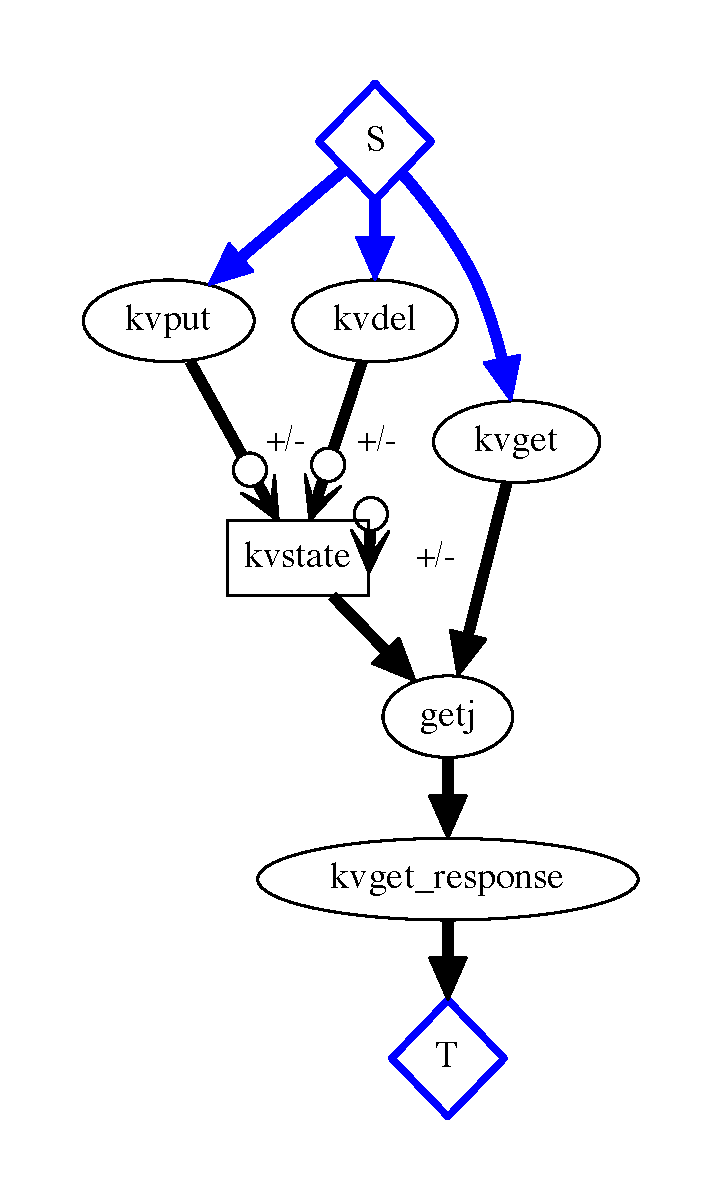
\includegraphics[width=0.7\linewidth]{kvs.pdf}
\end{minipage}

\vspace{-10pt}
\caption{A Bloom key-value store and its CALM visualization}
\label{fig:kvs}
\vspace{-2pt}

\end{figure}



\begin{figure}[t]
\begin{minipage}{.48\textwidth}
\footnotesize

%%\centering
\begin{tabular}{|l|l|l|}
\hline
Class & Label & Interpretation \\ \hline
Primitive & $\bot$ & Transformation does not affect consistency \\ \cline{2-3}
& $N$ & Nonmonotonic (order-sensitive) \\
& & transformation \\ \cline{2-3}
& $A$ & Asynchronous (order-sacrificing) \\
& & communication \\ \hline
Compound & $D$ & Diffluent (potentially different \\
& & results in different executions or on \\
& & different replicas) \\ \cline{2-3}
& $R$ & Restores order.  Represents some \\
& & coordination protocol. \\ \hline

\end{tabular}

%\vspace{-10pt}
%\caption{Consistency Labels}
%\label{fig:basic-labels}
%\vspace{-2pt}
%\end{figure}


%\begin{figure}[t]

\end{minipage}
\begin{minipage}{.48\textwidth}
\raggedleft

\footnotesize
\begin{tabular}{|l|l|}
\hline
Rule & Interpretation \\ \hline
$AN \rightarrow D$ & Loss of order followed by order-\\
&sensitivity causes diffluence \\ \hline
$D \alpha \rightarrow D$ & \\
$\alpha D \rightarrow D$ & Diffluence is final\\ \hline
$\bot \beta \rightarrow \beta$ & \\
$\beta \bot \rightarrow \beta$ & $\bot$ propagates labels from the left \\ \hline
$AR \rightarrow R$ & Order lost and regained \\ \hline
$RA \rightarrow A$ & $R$'s labors lost \\ \hline
$RN \rightarrow R$ & $N$ an do no harm \\ \hline
$NR \rightarrow N$ & $R$ can do no good \\ \hline

\end{tabular}
\end{minipage}
\vspace{-10pt}
\caption{Labels and Reduction Rules}
\label{fig:rules}
\vspace{-2pt}
\end{figure}


Figure~\ref{fig:rules} enumerates the Bloom consistency labels and rules for their propagation.
Consider again the overwriting key-value store presented in Figure~\ref{fig:kvs}.
CALM analysis detected nonmonotonic operations in the dataflow from \emph{kvput}
to \emph{kvget\_response}, because PUTs implicitly delete old values.  As we collapse the labels,
the nonmonotonic label will dominate, and we will ultimately associate with BasicKVS the following signature:
$kvget\_response: \{N(put) | \bot(get)\}$.
Consider now a larger system that uses the key-value store.  It will not be safe to attach an asynchronous
stream to the \emph{kvput} interface of the store, as this will lead to a divergent consistency label
(due to the rule $AN \rightarrow D$).  
Order must be \emph{restored} (via
interposition of a dataflow labeled ``R'') 
to asynchronous (i.e., unordered) inputs
before composing with \emph{kvput}.  This corresponds to intuition:
a key-value store with ``last writer wins'' semantics is highly sensitive to the order in which it receives writes.
If the KVS is replicated, we must be especially careful about reordering of writes, as this
may lead to inconsistent state on different replicas---indeed, we may be willing to pay a coordination
cost to totally order all writes.
Reads, on the other hand, may be reordered freely.

In practice, distributed systems are often composed from a large 
collection of functional units, loosely coupled using message-based APIs.
Such services are often implemented in a variety of programming 
languages, and in some cases they are opaque and outside the control of
the programmer using them.  
Many services (e.g. data stores and message queues) provide their own 
consistency guarantees, but how are we to reason about the consistency of an
\emph{application} that calls out to various such services and transforms
and combines their responses?  

The intuitions behind the CALM Theorem apply at this level of reasoning
just as they applied to the low-level composition of relational operators
in a Bloom execution.  Consider an inventory management application 
that makes calls into two asynchronously updated but
eventually consistent datastores.  It selects from the first service---an 
inventory datastore---the model numbers of all toaster ovens that are currently in stock.  For each, it probes the second datastore---a recall database---to
see if the unit has been recalled.  Finally, the application returns the 
set of model numbers for units that have \emph{not} been recalled.  Observe that this
application has a race condition due to the negation (``not recalled''): for a given model number $N$, the order of a request to lookup $N$ and a request to insert a recall for $N$ will determine whether or not the system returns $N$.  In a distributed implementation, both orderings could occur at different replicas, yielding inconsistent results.  If the orchestration
application that correlates the results from the different datastores were written in Bloom, we would observe that although the datastores are monotonic, 
the manner in which their results are \emph{used} is not.  If the inputs to 
the datastores are asynchronous (reorderable), then the output of the 
application may be inconsistent.  In the Bloom labeling system presented above, both services would be labeled 
``A''---that is, asynchronously updated but otherwise monotonic.  The orchestration code that connects them would be 
labeled ``N''---nonmonotonic, due to the negation.  The resulting composition would then be labeled ``D''---divergent, with
a point of order in the orchestration code that should be resolved (e.g., by versioning the recall database and issuing queries against the 
oldest ``complete'' version).


\subsection{Summary of Tasks and Goals}
\jmh{Make an explicit plan here to do something new with widely-used systems -- zookeeper+voldemort+something?  Perhaps talk about potential collaboration with LinkedIn.}

The labeling system presented above provides a framework for reasoning about service composition that is 
mostly independent of Bloom, so long as we can accurately attribute consistency labels to service APIs.
If the services are written in Bloom, we can derive their labels automatically---otherwise we may rely on annotations.
As the example above indicated, however, we must be very careful how we \emph{use} data returned from 
eventually consistent services
if we wish to assert that application output is likewise consistent.  Hence the ``glue'' language used
to compose services must also be amenable to CALM analysis and label propagation.

We are currently exploring the use of Bloom as a high-level service orchestration language.
As a proof of concept, we are collaborating with LinkedIn to implement a collection of services and applications atop
their Service-oriented Architecture.
We will show how CALM analysis can ease the burden of reasoning about the behavior of applications
that call out to a number of services (including data stores, message queues, coordination services like Zookeeper, 
and logging subsystems)
with various service-level consistency guarantees.
This project will rely on the following technology:

\begin{itemize}
\item \textbf{Path labeling and label propagation}.
We are currently developing a collection of ``consistency labels'' that 
can be used to describe the data flowing out of a given module.  When the module
is implemented in Bloom, we can derive these labels automatically via program
analysis of the low-level code.  Each individual transformation or rule is 
given a label, and chains of labels are ``collapsed'' based on CALM analysis to 
a single label for each module output.  
Otherwise, such labels can be associated with service APIs as an annotation.  
When two modules are composed, the label of the resulting composition is derived
by collapsing the labels of the component modules.
As programmers construct larger systems out of reusable modules, they may 
hide the complexity of module implementations while preserving those semantic 
details that may affect the consistency of future compositions. The 
labeling technique is a confluent term rewriting system that allows us to 
characterize any dataflow as a compact expression with an intuitive 
meaning in the context of distributed systems.

\item \textbf{Automated coordination synthesis}.

Given the labeling system described above, certain compositions will be 
labeled as inconsistent.  In such cases, we will exploit the CALM
analysis system to discover locations in an otherwise 
inconsistent dataflow where interposition of such an order-restoration 
coordination mechanism can yield an eventually consistent program.
We will provide a mechanism by which a programmer may either supply 
their own coordination protocol, or rely on the system to synthesize one. 
In the latter case, we will show that a generic coordination 
protocol---totally ordered broadcast---may be interposed into arbitrary 
programs at their ``points of order''
to ensure consistency of replicated state.

\item \textbf{Uniform error communication and handling}
A significant challenge for an orchestration language is robust error handling.
Calls to services can fail in various ways; in some cases services can report the error
back to the caller along with relevant information about its cause, while it other cases
applications must manage timeout and retry logic.  Since a robust orchestration language will
be fundamentally nondeterministic, we will have to revisit the consistency labeling system to
accomodate this uncertainty.

\end{itemize}

